\section[UserStories]{UserStories}
As \textsl{user stories} são requisitos funcionais a nível de time dentro do
\textsl{framework} SAFe. Eles são os épicos e as \textsl{features} com um nível
de abstração mais refinado.

Logo abaixo, foi exemplificado como uma história de usuário foi planejada na ferramenta de gerenciamento TargetProcess.

\begin{figure}[!htb]
    \centering
    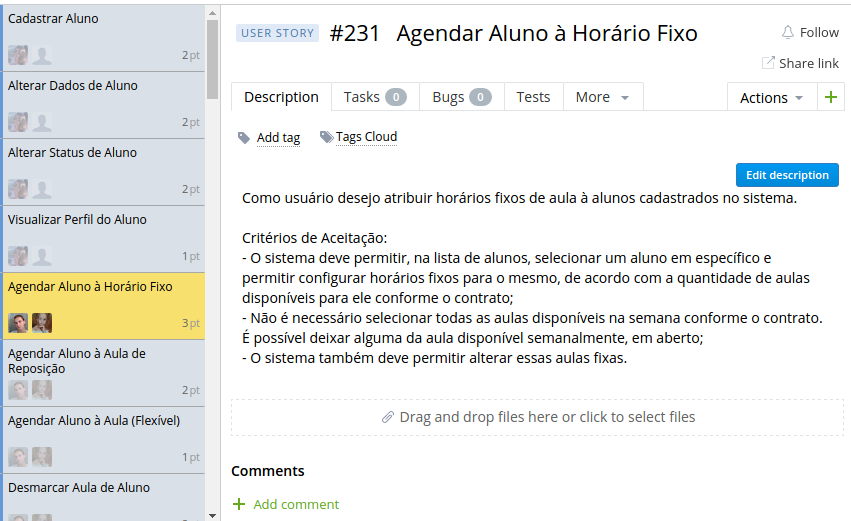
\includegraphics[width=\textwidth]{figuras/exemplo_user_story.png}
    \caption{Exemplo História de Usuário}
    \label{fig:exemplo_user_story}
\end{figure}

Em seguida, dos itens 1 ao 46 foram listadas as Histórias de Usuário requisitadas pela equipe de desenvolvimento.

\subsection[Visualizar Agenda Diária]{Visualizar Agenda Diária}
Eu como usuário administrador quero visualizar agenda diária para
me certificar de quais alunos tiveram ou terão acesso ao estabelecimento
em determinada data para aula.
\begin{quote}
    \textbf{Pontuação:} 2 pts
\end{quote}

\subsection[Visualizar Horário Específico]{VisualizarHorário Específico}
Eu como usuário administrador quero visualizar a agenda referente a um horário
específico para me certificar de quais alunos tiveram ou terão acesso ao
estabelecimento em determinado momento do dia para aula.
\begin{quote}
    \textbf{Pontuação:} 2 pts
\end{quote}

\subsection[Visualizar Agenda Semanal]{Visualizar Agenda Semanal}
Eu como usuário administrador quero visualizar a agenda semanal para assim me
certificar de quais alunos tiveram ou terão acesso ao estabelecimento durante tal
semana para aulas.
\begin{quote}
    \textbf{Pontuação:} 2 pts
\end{quote}

\subsection[Visualizar Agenda Mensal]{Visualizar Agenda Mensal}
Eu como usuário administrador quero visualizar a agenda mensal para me
certificar de quais alunos tiveram ou terão acesso ao estabelecimento durante
determinado mês para aulas.
\begin{quote}
    \textbf{Pontuação:} 2 pts
\end{quote}

\subsection[Gerar Relatório Diário de Aulas]{Gerar Relatório Diário de Aulas}
Eu como usuário administrador quero gerar um relatório diário de aulas para me
certificar de quais alunos compareceram ou não a aula agendada.
\begin{quote}
    \textbf{Pontuação:} 2 pts
\end{quote}

\subsection[Criar Aulas]{Criar Aulas}
Essa história de usuário tem como objetivo o desenvolvimento da \textsl{model} referente
a Aulas. Assim permitindo que sejam feitas dependências internas entre aluno
e aulas.
\begin{quote}
    \textbf{Pontuação:} 2 pts
\end{quote}
\begin{quote}
\textbf{Critérios de aceitação:}
    \begin{itemize}
        \item O sistema deve permitir registrar novas aulas.
    \end{itemize}
\end{quote}

\subsection[Cadastrar Plano de Contrato]{Cadastrar Plano de Contrato}
Eu como usuário administrador quero cadastrar planos de contratos com as
informações de: quantidade de vezes por semana, período do plano em meses,
valor mensal e percentual de desconto baseado no plano de 1 mês.
\begin{quote}
    \textbf{Pontuação:} 3 pts
\end{quote}
\begin{quote}
\textbf{Critérios de Aceitação:}
    \begin{itemize}
        \item O sistema deve permitir a edição de um ou mais dados de planos de contrato
        como o preço da mensalidade e o desconto.
    \end{itemize}
\end{quote}

\subsection[Submeter Contrato]{Submeter Contrato}
Eu como usuário administrador quero realizar o \textsl{upload} de contratos nos formatos
PDF, doc com seu respectivo título e descrição para que eu possua um controle
sobre os antigos contratos e possa imprimir os atuais.
\begin{quote}
    \textbf{Pontuação:} 0 pts
\end{quote}

\subsection[Visualizar Contrato]{Visualizar Contrato}
Eu como usuário administrador quero visualizar a lista dos documentos hospedados
(listados pelo seu respectivo título) e abrir esses documentos para que eu possa
visualizar uma lista dos arquivos disponíveis no sistema e realizar o \textsl{download}
de cada um deles.
\begin{quote}
    \textbf{Pontuação:} 0 pts
\end{quote}

\subsection[Remover Contrato]{Remover Contrato}
Eu como usuário administrador quero remover do sistema os contratos hospedados
para que eu possa remover os que não são mais importantes e possua controle
sobre os contratos.
\begin{quote}
    \textbf{Pontuação:} 0 pts
\end{quote}

\subsection[Cadastrar Professor]{Cadastrar Professor}
Eu como usuário administrador quero cadastrar os professores no sistema para
que possa ter um registro com as informações dos professores e maior controle
sobre eles.
\begin{quote}
    \textbf{Pontuação:} 2 pts
\end{quote}

\subsection[Alterar Dados de Professor]{Alterar Dados de Professor}
Eu como usuário administrador quero alterar dados dos professores no sistema
para que possa atualizar o registro que contém as informações sobre eles.
\begin{quote}
    \textbf{Pontuação:} 2 pts
\end{quote}

\subsection[Alterar Status de Professor]{Alterar Status de Professor}
Eu como usuário administrador quero registrar no sistema se o professor está
ativo ou não no estúdio de pilates, a fim de controlar a alocação de
professores em horários de aulas e permitir ou rejeitar o seu acesso ao sistema.
\begin{quote}
    \textbf{Pontuação:} 1 pt
\end{quote}

\subsection[Cadastrar Saídas]{Cadastrar Saídas}
Eu como usuário administrador quero cadastrar as saídas(despesas) da empresa para que
possa manter um histórico financeiro da empresa.
Exemplo: Contas de água, luz, telefone, internet, impostos.
\begin{quote}
    \textbf{Pontuação:} 2 pts
\end{quote}

\subsection[Editar Saídas]{Editar Saídas}
Eu como usuário administrador quero editar as saídas(despesas) da empresa para que possa
corrigir qualquer eventual equívoco ou falta de informações associadas ao
histórico financeiro da empresa.
\begin{quote}
    \textbf{Pontuação:} 2 pts
\end{quote}

\subsection[Visualizar Saída]{Visualizar Saída}
Eu como usuário administrador quero visualizar as saídas(despesas) da empresa
para que possa analisar o fluxo de caixa da empresa.
\begin{quote}
    \textbf{Pontuação:} 1 pt
\end{quote}

\subsection[Visualizar Receita]{Visualizar Receita}
Eu como usuário administrador quero visualizar as entradas e saídas(despesas) da empresa
para que possa analisar o fluxo de caixa da empresa.
\begin{quote}
    \textbf{Pontuação:} 1 pt
\end{quote}

\subsection[Gerar Relatório de Entradas]{Gerar Relatório de Entradas}
Eu como usuário administrador quero gerar um relatório que especifique as
entradas da empresa para que possa melhor gerencia-la e verificar o quanto de
dinheiro foi obtido pela empresa.
\begin{quote}
    \textbf{Pontuação:} 3 pts
\end{quote}

\subsection[Visualizar Entradas]{Visualizar Entradas}
Eu como usuário administrador quero visualizar as entradas para que possa
verificar o quanto de dinheiro foi obtido pela empresa.
\begin{quote}
    \textbf{Pontuação:} 1 pt
\end{quote}

\subsection[Agendar Aluno à Horário Fixo]{Agendar Aluno à Horário Fixo}
Eu como usuário administrador quero atribuir horários fixos de aula à alunos
cadastrados no sistema.
\begin{quote}
    \textbf{Pontuação:} 3 pts
\end{quote}

\subsection[Agendar Aluno à Aula de Reposição]{Agendar Aluno à Aula de Reposição}
Eu como usuário administrador quero atribuir novo horário a alunos que solicitam
reposição de aula.
\begin{quote}
    \textbf{Pontuação:} 2 pts
\end{quote}
\begin{quote}
\textbf{Critérios de Aceitação:}
    \begin{itemize}
        \item Ao selecionar a aula de algum aluno, deve ser possível criar uma nova aula,
        que será aula de reposição, transformando a aula atual em aula cancelada;
        \item Indicar a data da aula que está sendo reposta.
    \end{itemize}
\end{quote}

\subsection[Agendar Aluno à Aula]{Agendar Aluno à Aula}
Eu como usuário administrador quero atribuir um aluno a determinado
horário/aula quando necessário.
\begin{quote}
    \textbf{Pontuação:} 1 pt
\end{quote}

\subsection[Desmarcar Aula de Aluno]{Desmarcar Aula de Aluno}
Eu como usuário administrador quero cancelar aula de determinado aluno quando
necessário.
\begin{quote}
    \textbf{Pontuação:} 2 pts
\end{quote}

\subsection[Remarcar Aula de Aluno]{Remarcar Aula de Aluno}
Eu como usuário administrador quero remarcar aulas referentes a determinado
aluno quando necessário. Como por exemplo mudar aula de um dia para outro,
tanto pra dias anteriores como posteriores, mas já com uma data definida
para fazer a aula.
\begin{quote}
    \textbf{Pontuação:} 2 pts
\end{quote}

\subsection[Conferir Aulas Remanescentes]{Conferir Aulas Remanescentes}
Eu como usuário administrador quero conferir as aulas restantes de cada aluno.
\begin{quote}
    \textbf{Pontuação:} 1 pt
\end{quote}

\subsection[Conferir Aulas Realizadas]{Conferir Aulas Realizadas}
Eu como usuário administrador quero conferir as aulas realizadas por alunos.
\begin{quote}
    \textbf{Pontuação:} 1 pt
\end{quote}

\subsection[Agendar Aula Experimental]{Agendar Aula Experimental}
Eu como usuário administrador quero agendar aula experimental quando necessário.
\begin{quote}
    \textbf{Pontuação:} 1 pt
\end{quote}
\begin{quote}
\textbf{Critérios de Aceitação:}
    \begin{itemize}
        \item O sistema deve permitir criar uma aula experimental quando necessário direto
        no menu das aulas existentes.
        \item É necessário apenas o nome e o telefone do aluno que irá fazer a aula
        experimental.
    \end{itemize}
\end{quote}

\subsection[Atribuir Falta de Aluno à Aula Marcada]{Atribuir Falta de Aluno à Aula Marcada}
Eu como usuário administrador quero atribuir uma falta a um aluno quando não
houver aviso prévio.
\begin{quote}
    \textbf{Pontuação:} 1 pt
\end{quote}

\subsection[Conferir Aulas de Reposição de Aluno]{Conferir Aulas de Reposição de Aluno}
Eu como usuário administrador quero conferir quantas aulas referentes a
reposição (aulas desmarcadas) o aluno possui.
\begin{quote}
    \textbf{Pontuação:} 1 pt
\end{quote}

\subsection[Conferir Aulas Perdidas de Aluno]{Conferir Aulas Perdidas de Aluno}
Eu como usuário administrador quero conferir a quantidade de faltas que o aluno
possui.
\begin{quote}
    \textbf{Pontuação:} 1 pt
\end{quote}

\subsection[Colocar Aluno na Lista de Espera]{Colocar Aluno na Lista de Espera}
Eu como usuário administrador quero colocar um aluno na lista de espera quando o
mesmo estiver esperando por um horário específico enquanto não houver vaga.
\begin{quote}
    \textbf{Pontuação:} 5 pts
\end{quote}

\subsection[Alterar Horário de Aula de Aluno]{Alterar Horário de Aula de Aluno}
Eu como usuário administrador quero alterar o horário de aula de um aluno no
mesmo dia.
\begin{quote}
    \textbf{Pontuação:} 2 pt
\end{quote}

\subsection[Adicionar Plano de Contrato ao Aluno]{Adicionar Plano de Contrato ao Aluno}
Eu como usuário administrador quero associar um plano de contrato a um aluno.
\begin{quote}
    \textbf{Pontuação:} 1 pt
\end{quote}
\begin{quote}
\textbf{Critérios de Aceitação:}
    \begin{itemize}
        \item O sistema deve permitir com que os contratos sejam relacionados ao cliente. Ao realizar essa ligação, outras informações como Descontos, data de início, deve ser salvas. Posteriormente, essa tabela de ligação estará relacionada a uma segunda tabela de pagamentos. Além disso, o ultimo plano deve ser "ativo" quando criado e os planos anteriores desativados;
        \item As informações inseridas pelo usuário serão: desconto, data de início e o plano de contrato.
    \end{itemize}
\end{quote}

\subsection[Renovar Plano de Aluno]{Renovar Plano de Aluno}
Eu como usuário administrador quero renovar o plano de contrato de aluno ao fim do contrato do mesmo.
\begin{quote}
    \textbf{Pontuação:} 1 pt
\end{quote}
\begin{quote}
\textbf{Critérios de Aceitação:}
    \begin{itemize}
        \item O sistema deve permitir a renovação do plano de um aluno.  Os contratos renovados devem possuir todos os atributos iguais exceto a data de início do contrato, que deve ser o dia atual.
    \end{itemize}
\end{quote}

\subsection[Visualizar Vencimento de Plano de Aluno]{Visualizar Vencimento de Plano de Aluno}
Eu como usuário administrador quero visualizar quando o plano de determinado
aluno irá vencer.
\begin{quote}
    \textbf{Pontuação:} 1 pt
\end{quote}
\begin{quote}
\textbf{Critérios de Aceitação:}
    \begin{itemize}
        \item Ao verificar os planos de contrato de um aluno, o sistema deve informar que dia é o vencimento do plano. Caso o plano já tenha vencido ou seja inexistente, essa informação deve ser mostrada ao usuário.
    \end{itemize}
\end{quote}

\subsection[Gerar Relatório Mensal com o Vencimentos Planos]{Gerar Relatório Mensal com o Vencimentos Planos}
Eu como usuário administrador quero gerar um relatório mensal onde seja possível
saber quais planos referentes a quais alunos devem vencer no mês.
\begin{quote}
    \textbf{Pontuação:} 2 pts
\end{quote}
\begin{quote}
\textbf{Critérios de Aceitação:}
    \begin{itemize}
        \item O usuário seleciona qual mês e ano deseja consultar os planos que vencerão. Após essa seleção o sistema deve retornar como resultado quais planos dos clientes vencerão no mês e ano selecionado. A opção padrão deve ser a do mês e ano atual.
    \end{itemize}
\end{quote}

\subsection[Enviar Notificações de Vencimento para o Aluno]{Enviar Notificações de Vencimento para o Aluno}
Eu como usuário administrador quero que sejam enviadas notificações aos alunos,
de forma automatizada, sobre o vencimento da sua mensalidade e/ou plano.
\begin{quote}
    \textbf{Pontuação:} 2 pts
\end{quote}

\subsection[Gerar Relatório Mensal com os Alunos Ativos]{Gerar Relatório Mensal com os Alunos Ativos}
Eu como usuário administrador quero gerar um relatório mensal onde eu posso me
certificar dos alunos ainda ativos no sistema.
\begin{quote}
    \textbf{Pontuação:} 2 pts
\end{quote}

\subsection[Cancelar Plano de Contrato de Aluno]{Cancelar Plano de Contrato de Aluno}
Eu como usuário administrador quero cancelar o plano de contrato de um aluno,
ou seja, fazer a recisão do mesmo.
\begin{quote}
    \textbf{Pontuação:} 3 pts
\end{quote}
\begin{quote}
\textbf{Critérios de Aceitação:}
    \begin{itemize}
        \item O sistema deve permitir o cancelamento do plano de um aluno. Após cancelar o contrato, deve noticiar o usuário que essa operação foi realizada. Os contratos cancelados devem continuar salvos no banco de dados.
    \end{itemize}
\end{quote}

\subsection[Alterar Plano]{Alterar Plano}
Eu como usuário administrador do sistema eu desejo cancelar o plano de um aluno e adicionar outro.
\begin{quote}
    \textbf{Pontuação:} 3 pts
\end{quote}
\begin{quote}
\textbf{Critérios de Aceitação:}
    \begin{itemize}
        \item O sistema deve permitir a mudança do plano de um aluno, seja na quantidade de vezes por semana ou no período do plano.
    \end{itemize}
\end{quote}

\subsection[Cadastrar Aluno]{Cadastrar Aluno}
Eu como usuário administrador quero cadastrar novos alunos no sistema.
\begin{quote}
    \textbf{Pontuação:} 2 pts
\end{quote}
\begin{quote}
\textbf{Critérios de Aceitação:}
    \begin{itemize}
        \item O sistema deve permitir o cadastro de clientes com os dados: nome, profissão, data de nascimento, endereço, CEP, telefone residencial, celular, e-mail, CPF, RG e status.
    \end{itemize}
\end{quote}

\subsection[Alterar Dados de Aluno]{Alterar Dados de Aluno}
Eu como usuário administrador quero alterar os dados cadastrais dos alunos a fim
de manter um registro atualizado deles.
\begin{quote}
    \textbf{Pontuação:} 2 pts
\end{quote}
\begin{quote}
\textbf{Critérios de Aceitação:}
    \begin{itemize}
        \item O sistema deve permitir a edição de um ou mais dados de clientes como: nome,
        profissão, data de nascimento, endereço, CEP, telefone residencial, celular,
        e-mail, CPF e RG.
    \end{itemize}
\end{quote}

\subsection[Alterar Status de Aluno]{Alterar Status de Aluno}
Eu como usuário administrador quero ativar ou inativar um aluno no sistema
quando chegar ao fim de seu plano de contrato, de acordo com a renovação ou não.
\begin{quote}
    \textbf{Pontuação:} 2 pts
\end{quote}
\begin{quote}
\textbf{Critérios de Aceitação:}
    \begin{itemize}
        \item O sistema deve permitir a edição do \textsl{status} (ativo/não ativo) de um aluno
        previamente selecionado.
    \end{itemize}
\end{quote}

\subsection[Visualizar Perfil de Aluno]{Visualizar Perfil de Aluno}
Eu como usuário administrador quero visualizar o perfil do aluno que contém suas
informações pessoais e plano de contrato.
\begin{quote}
    \textbf{Pontuação:} 1 pt
\end{quote}
\begin{quote}
\textbf{Critérios de Aceitação:}
    \begin{itemize}
        \item O sistema deve mostrar os dados do cliente: nome, profissão, data de nascimento, endereço, CEP, telefone residencial, celular, e-mail, CPF, RG e status;
        \item O sistema deve mostrar as informações referentes ao plano do cliente ativo no momento (Início do contrato, duração,  custo e descrição). Caso nenhum plano esteja ativo ou esse cliente não esteja associado a um contrato, deve ser mostrado na tela "Contrato vencido ou inexistente."
    \end{itemize}
\end{quote}

\subsection[Gerar Relatório com os Aniversariantes do Mês]{Gerar Relatório com os Aniversariantes do Mês}
Eu como usuário administrador quero visualizar a data de aniversário de todos os
alunos aniversariantes do mês para que possa desejá-los feliz aniversário.
\begin{quote}
    \textbf{Pontuação:} 2 pts
\end{quote}
\begin{quote}
\textbf{Critérios de Aceitação:}
    \begin{itemize}
        \item O usuário seleciona qual mês deseja consultar os aniversariante. Após essa seleção o sistema deve retornar como resultado com os clientes aniversariantes do mês selecionado. A opção padrão deve ser a do mês atual.
    \end{itemize}
\end{quote}

\subsection[Buscar Alunos no Sistema]{Buscar Alunos no Sistema}
Eu como usuário administrador quero pesquisar alunos por nome.
\begin{quote}
    \textbf{Pontuação:} 1 pt
\end{quote}
\begin{quote}
\textbf{Critérios de Aceitação:}
    \begin{itemize}
        \item O sistema deve mostrar a lista de clientes que contenha um nome ou pedaço de
        nome, digitado em um campo existente;
        \item Dentro da busca o sistema deve permitir clicar para editar os clientes que
        apareceram.
    \end{itemize}
\end{quote}
